\section{Methods and Materials}

\subsection{Dataset presentation} 

We focus on two data sets. The first one is PEPSI, a compilation of synthetic flow observations generated from outputs of various hydraulic flow models. This dataset is composed of 55525 observations from 29 rivers worldwide with 21 explanatory variables for each of them.

\noindent The main explanatory variables that we use for the statistic description of this dataset are : 
\begin{description}
    \item [- river]: river name
    \item [- day]: simulation day 
    \item [- reach]: reach index
    \item [- flowacc] : flow accumulation, i.e. size of the upstream watershed
    \item [- height]: free surface height
    \item [- W]: free surface top width
    \item [- A]: cross-sectional flow area
    \item [- S]: free surface slope 
    \item [- dA]: cross-sectional flow area above A0
    \item [- K]: Strickler value, computed by inverting Manning equation with parameters Q, A0, dA, W and S from the database
    \item [- A0]: unobserved cross-sectional flow area 
    \item [- Abar]: mean cross-sectional flow area  data
    \item [- Fr]: Froude number 
    \item [- U]: flow velocity 
    \item [- Q]: discharge 
\end{description}

The second dataset is HydroSwot, a database generated from observations -- from 153 rivers -- taken in-situ in North America. It contains 16638 observations with 41 explanatory variables.

Among the 41 measurements, the majority is not used for the statistic description. The important variables are the same as the ones for PEPSI, adding:

\begin{description}
    \item [- stage]
    \item [- dH]: water depth above unobserved flow
    \item[- PA]: mean annual precipitation
    \item[- TA]: mean annual temperature
\end{description}


\subsection{Dataset modifications}\\
First we clean our datasets. We delete all observations with NaN values, i.e. missing values.\\

In the Hydroswot dataset, we can find different names for the same river because of text processing when creating the data. We update the names to have each rivers with a single name and make easier the analysis. We obtain 134 rivers.  \\

The satellite does not detect small rivers with a width less than $80m$. Thus, we delete observation with a width under $80m$. We also remove observations with a river flow under $100 m^3/s$ because we assume they are too small rivers.\\

We remove the calculations of base streamflow, mean discharge quantile and floor composition from the Hydroswot base. We also remove the flow velocity, $U$, in the two datasets because having $U$ is a problem which is as difficult to resolve as having $Q$. As a matter of fact, this variable is linked with $Q$, with $Q = AU$.   \\

Finally, for PEPSI we obtain a dataset with 29 rivers, 51269 observations for 20 variables and for Hydroswot with 134 rivers, 11851 observations for 21 variables. \\
        
Due to previous modifications, for 10 sites in the HydroSwot dataset, we have only one observation. We cannot use these data because the variables $dA$ and $dH$ are calculated by differences, so we must have at least 2 observations to give them meaning. Hence, We remove these 13 observations. \\

\newpage
\subsection{Correlations, PCA}

We seek to determine which variables are most related to the discharge, and which best describe the characteristics of a river. First, we compute the correlations between all our variables, except the flow velocity \textit{U} and the different quantiles of discharge \textit{Qi\_GSCD} that are obviously highly linked with the discharge. The correlation is the relationship between two random quantitative variables which explains how they are linearly related. It is defined by :
\begin{equation}
    Cor(\underline{x},\underline{y}) = \frac{Cov(\underline{x},\underline{y})}{\sqrt{Var(\underline{x})Var(\underline{y})}}
\end{equation}
where \underline{x} and \underline{y} denote the samples of the two variables, $Cov$ the covariance between them, and $Var$ their respective variance. The correlation varies between $-1$ when the variables vary in strong opposite directions, and $1$ when they vary exactly in the same direction. Here, we use a correlation matrix to easily summarise all the correlations between all variables : one cell of the matrix represents the correlation between the row variable and the column one. Thus, the diagonal is full of $1$s, as it represents the correlation between a variable and itself.\newline

Second, we perform a Principal Component Analysis (PCA). The goal is to reduce the large shape of our problem by gathering our variables within metavariables to analyse our data more easily. The first step consists in a normalization of the data because of the different scales (understand units) of our variables. Then, we compute linear combinations of our initial variables. One linear combination represents one principal component or direction. The aim is to find which direction maximises the amount of variance of the data, i.e. the direction that captures most information of the data. 

Let $\Sigma$ be the covariance matrix associated to the normalized data. Computing the principal component \textbf{amounts to find} the eigenvector $a_1$ associated to the largest eigenvalue of $\Sigma$ denoted as $\lambda_1$, i.e. to solve the following equation :
\begin{equation}
    \Sigma a_1 = \lambda_1 a_1
\end{equation}
Thus, we get the principal components by order of significance by ranking the eigenvectors according to the values of their associated eigenvalues. Then, we select the number of axes which is necessary to capture the majority of the information. A well-known rule is to keep the first $n$ components such as the sum of their variances reaches $80\%$ of the total variance.

Finally, we interpret our PCA with two different types of graph. The first one is the loading plot: all the variables of the problem are displayed in the spans formed by each pair of principal components retained. The aim is to find how the initial variables are related with the principal components. The second plot is the score plot, which plots the individuals' coordinates in the the same spans as mentioned above. We then can observe clusters of individuals.

\subsection{Clustering - K-means}

K-means is unsupervised classification method method to define clusters in a dataset. We first have to find the best number $k$ of clusters to give to the algorithm. Then, it works as follows.

First, $k$ class centers, called centroids, are randomly initialized. Second, individuals are assigned to the class whose center is closest, according to the chosen distance metric. Here, we use the Euclidean metric. Third, the centers of gravity of each class are computed. Finally, we repeat second and third instructions until the algorithm's convergence.

One edge of the K-means algorithm is that we are sure to obtain a convergence of it. Nonetheless, we obtain different classes depending on the random initialization at the beginning. To overcome that problem, the algorithm will be run with different centroid seeds, and the final results will be the best output in terms of inertia.
 
\subsection{Artifical Neural Networks}

The prior methods and materials described are essential to use artificial neural networks (ANN). 

An artificial neural network is non linear with respect to its parameters, noted as $\theta$, that associates to an entry $x$ an output $y = f (x, \theta)$. In this study, our output is unidimensional but it can be multidimensional in other applications. \newline

\textbf{An artificial neuron}, inspired by a biological neuron, is composed of : 
\begin{itemize}
    \item[\textbullet] a function $f_j$ of the input $x = \{x_1 \mbox{, ... , }x_d\}$
    \item[\textbullet] a vector of connection weights $w_j = \{w_{j,1} \mbox{, ... , } w_{j,d}\}$
    \item[\textbullet] a neuron bias noted $b_j$
    \item[\textbullet] an activation function $\phi_j$
\end{itemize}

This give us $y_j = f_j(x) = \phi ( <w_j , x> + b_j )$. Figure \ref{fig:neuron} represents an artificial neuron. $\Sigma$ corresponds to $<w_j,x> + b_j$. 

\begin{figure}[H]
    \centering
    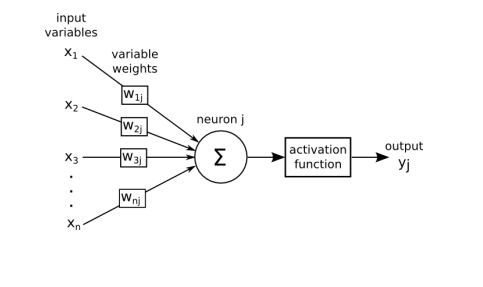
\includegraphics{Graph/neuron.png}
    \caption{Schematic representation of an artificial neuron
}
    \label{fig:neuron}
\end{figure}



\textbf{A neural network}, represented in figure \ref{fig:neural_network}, is an association of several neurons, grouped in layers, called hidden layers. In this structure, also known as a multi-layer perceptron, the output of each neuron of a layer becomes the input of the neurons of the next layer. A potential different activation function than the hidden layers may be applied on the output layer depending on the problem, classification or regression. After having defined the architecture, we have to estimate the parameters, $w_j$ and $b_j$, with a training sample and the back propagation algorithm. 
\begin{figure}[H]
    \centering
    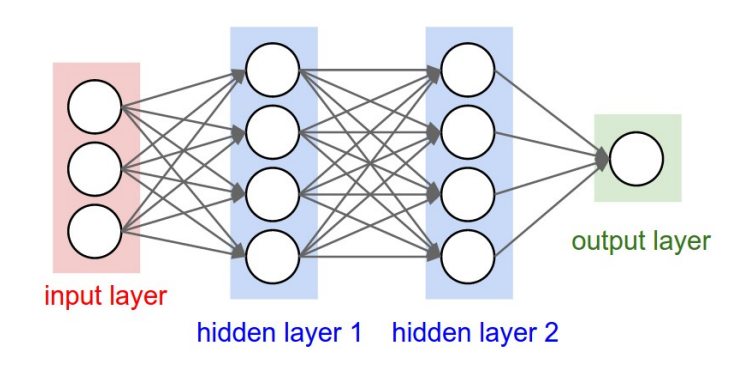
\includegraphics[scale = 0.7]{Graph/neural_net.png}
    \caption{A neural network architecture}
    \label{fig:neural_network}
\end{figure}

A neural network is executed as follow : 
\begin{itemize}
    \item We select the explanatory variables used to train the network. The input data needs to be scaled whereas the output - the flow in our case - does not need to be scaled. Then we split our dataset into a training set and a test set, with a proportion of $80-20\%$.
    \item We choose a loss function. The main loss functions that we will use are Mean Absolute Error (MAE) and Mean Square Error (MSE).
    \item We randomly initialize the parameters $W$ and $b$. 
    \item We set $h^{(0)}(x) = x$. We compute at each hidden layer $k$, $h^{(k)}(x) = \phi (Wh^{(k-1)}(x)+b^{(k)})$ where $x$ is the input data. Then we compute the predicted values. This is the \textit{forward} phase. 
    \item We minimize the loss function, generally with a gradient descent algorithm. The gradient is computed with the back propagation algorithm and the backpropagation equations.  This is computed on subsets, called batch,  because of the size of the datasets. Then, the values obtained are used to update the parameters. This is the \textit{backward} phase. 
    \item We iterate the \textit{forward} and the \textit{backward} phases a number of times called $epochs$ that we define. 
\end{itemize}


\textbf{- Mieux expliquer concept de batch ? 
- Détailler back propgation algorithm ? Parler de la théorie derrière ? } \\




The success of the method came from a universal approximation theorem due to Cybenko (1989) and Hornik (1991). Le Cun (1986) proposed an efficient way to compute the gradient of a neural network, called backpropagation of the gradient, that allows to obtain a local minimizer of the quadratic criterion easily.
\newline



\subsection{Long Short-Term Memory Networks}

Long short-term memory (LSTM) has been introduced by Sepp Hochreiter and Jürgen Schmidhuber in 1997 \cite{lstm_createur}. 

The main quality of a LSTM network and a recurrent neural network (RNN) is that they can manage the time dependance contrary to classical neural networks. \\

To compute a RNN we have to choose the number of memory layers, $K$. If $K$ is too big, the number of parameters increases too much. It becomes too complicated to learn the weights due to the vanishing gradient. RNN does not have a long term memory. In our case we need a long term memory. We must use LSTM networks. \\

A LSTM includes an input gate, an output gate and a forget gate. A LSTM has his own memory $c$. Figure \ref{fig:lstm cell} shows the architecture at time $t$ of a LSTM cell.

\begin{figure}[H]
    \centering
    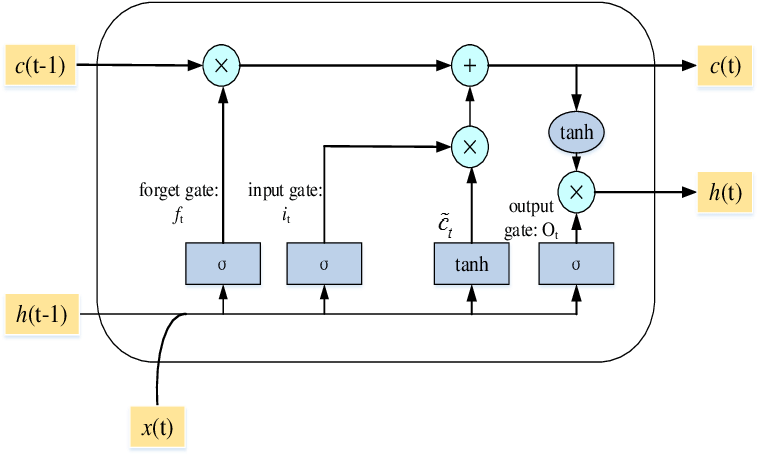
\includegraphics[scale = 0.4]{Graph/cellule_lstm.png}
    \caption{LSTM cell}
    \label{fig:lstm cell}
\end{figure}

$\bullet$ The forget gate is used to "forget" useless information. $f_t = \sigma(W, [h(t-1), x(t)] + b_f)$ \\
\indent $\bullet$ The input gate proposes new information to put into the cell memory. $\tilde{C}_t = tanh(W, [h(t-1), x(t)] + b_f)$ corresponds to what information we will put into the cell memory. $i_t = \sigma(W, [h(t-1), x(t)] + b_f)$ corresponds to the quantity of information we will add.\\
\indent $\bullet$ We use the two previous gates to compute the cell memory : $c(t) = c(t-1) f_t + i_t \tilde{C}_t $\\
\indent $\bullet$ The output gate : $h(t) = \sigma(W, [h(t-1), x(t)] + b_f) tanh(c(t)$. It defines the output of the cell using the cell memory $c(t)$ and a function which determines what information to take from the memory.\\


\noindent $\sigma$ is the sigmoid function.\\
$\{..., x_{t-1}, x_t, x_{t+1}, ... \}$ is the input time series. 

LSTM are linked in the way showed in figure \ref{fig:schema lstm}. \\

\begin{figure}[H]
    \centering
    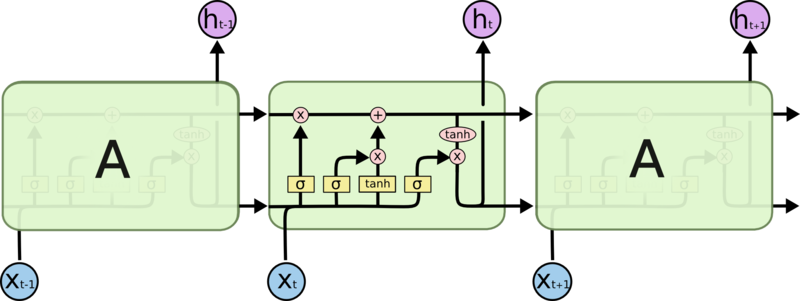
\includegraphics{Graph/schema_lstm.png}
    \caption{LSTM schema}
    \label{fig:schema lstm}
\end{figure}

In this illustration, we have 3 LSTM cells. 


\subsection{Performance criteria}

To evaluate the performances of a neural network, we quantify the errors thanks to different criteria.

\subsubsection{Useful common metrics}
 We compute the \textit{Mean Square Error}, denoted by $MSE$, and defined in (\ref{eq:mse}).
\begin{equation}
    MSE(y) = {\frac{1}{n} \left( \sum^n_{i=1}(y^{est}_i - y^{obs}_i)^2 \right)}
    \label{eq:mse}
\end{equation}
with $y^{est}_i$ the $i^{th}$ estimation and $y^{obs}_i$ the true value associated.\\

\textit{Mean Absolute Error}, denoted by $MAE$ has a physical meaning, as it does not modify the values of the river discharge. Using the same notations as previous, $MAE$ is defined in (\ref{eq:mae}).
\begin{equation}
    MAE(y) = {\frac{1}{n} \left( \sum^n_{i=1}\lvert y^{est}_i - y^{obs}_i\rvert \right)}
    \label{eq:mae}
\end{equation}

 The \textit{Pearson correlation coefficient}, denoted by $R2$ is set in (\ref{eq:r2}).
\begin{equation}
    R2(y) = \frac{\sum_{i=1}^{n}(y^{est}_i - \bar y^{est}) (y^{obs}_i - \bar y^{obs})} {\left(\sum_{i=1}^{n}(y^{est}_i - \bar y^{est})^2\right)^{1/2}\left(\sum_{i=1}^{n}(y^{obs}_i - \bar y^{obs})^2\right)^{1/2}}
    \label{eq:r2}
\end{equation}

where $\bar y^{est}$ the average value of the estimations and $\bar y^{obs}$ the average value of the validation values. 

We define the \textit{Root Mean Square Error} in (\ref{eq:rmse}), denoted by $RMSE$ and the \textit{Normalized Root Mean Square Error}, denoted by $nRMSE$ in (\ref{eq:nrmse}).
\begin{equation}
    RMSE(y) = \sqrt {\frac{1}{n} \left( \sum^n_{i=1}(y^{est}_i - y^{obs}_i)^2 \right)}
    \label{eq:rmse}
\end{equation}

\begin{equation}
    nRMSE(y) = \frac{RMSE(y)} {\bar y^{obs}}
    \label{eq:nrmse}
\end{equation}

\subsubsection{Useful metrics in hydrology}

Then, we define two other metrics specific to hydrology. The first one is the \textit{Nash-Sutcliffe model Efficiency}, denoted by $NSE$ and defined in (\ref{eq:nse}) with the same notations defined in section $2.7.1$. The second one is the \textit{Kling-Gupta model Efficiency}, denoted by $KGE$ in (\ref{eq:kge}).
\begin{equation}
    NSE(y) = 1 - \frac{\sum^n_{i=1}(y^{est}_i - y^{obs}_i)^2} {\sum^n_{i=1}(y^{obs}_i - \bar y^{obs})^2}
    \label{eq:nse}
\end{equation}


\begin{equation}
    KGE(y) = 1 - \sqrt {(\beta_{KG}-1)^2+(\alpha_{KG}-1)^2+(R^2-1)^2}
    \label{eq:kge}
\end{equation}
where $\beta_{KG}=\frac{\bar y^{est}}{\bar y^{obs}}$ and $\alpha_{KG} = \frac{\sigma(y^{est})}{\sigma(y^{obs})}$.

\subsubsection{Physical criteria : Low-Froude}

The last criteria we define is the Low-Froude model. The objective is to match physical criteria with a neural network. In our case we want to know if the predicted river flow follows the Low-Froude model. Its definition is the following :
\begin{equation}
    Q^{3/5}_{r,p} = \alpha_r^{3/5} ( c_{r,p}^{(1)} A_{0,r} + c_{r,p}^{(2)})(c_{r,p}^{(4)}A_{0,r} + c_{r,p}^{(3)})^{3/5\beta_r}
    \label{eq:low froude}
\end{equation}
where : $ c_{r,p}^{(1)} = W_{r,p}^{-2/5}S_{r,p}^{3/10}$, $ c_{r,p}^{(2)} = c_{r,p}^{(1)} \partial A_{r,p}$, $ c_{r,p}^{(3)} = (H_{r,p} - H_{r,0})$, and  $ c_{r,p}^{(4)} = \frac{1}{W_{r,0}}$.


